\documentclass[letter]{article}
\renewcommand{\baselinestretch}{1.25}

\usepackage[margin=1in]{geometry}
\usepackage{physics}
\usepackage{amsmath}
\usepackage{graphicx}
\usepackage{pythonhighlight}

\allowdisplaybreaks

%opening
\title{MECH 6327 - Homework 2}
\author{Jonas Wagner}
\date{2021, February 22}

\begin{document}

\maketitle


\section{Problem Set 1: Convex Sets}

\subsection{Problem 2.5}
\textbf{Problem:}\\
What is the distance between two parallel hyperplanes: $\{x \in \real^n | a^T x = b_1\}$ and $\{x \in \real^n | a^T x = b_2\}$?\\

\noindent
\textbf{Solution:}\\
Under the assumption that $a\in \real^n$ and $b_1,b_2 \in \real$, the quantity $a^T x_0$ represents the component of $x_0$ in the normal direction. Similarly, the quantities $b_1$ and $b_2$ represent the euclidean distance of the hyperplane from the origin (in the normal direction). Since the hyperplanes are parrellel, the distance between them is the difference between their offsets:
\begin{equation}
	\text{Distance between hyperplanes: } b_1 - b_2
\end{equation}


\subsection{Problem 2.7}
\textbf{Problem:}\\
\textit{Voronoi description of halfspace.} Let $a$ and $b$ be distinct points in $\real^n$. Show that the set of all points that are closer to $a$ than $b$ via the euclidean norm is a halfspace. Describe it explicitly as an inequality and draw a picture.

\noindent
\textbf{Solution:}\\
The set of all points closer to $a$ then $b$ can be defined as:
\begin{equation}
	\{x \in \real^n \ | \ \norm{x-a}_2 \leq \norm{x-b}_2\}
\end{equation}

The boundary defining this halfspace will be a plane defined by the normal vector $c$ representing the distance between $a$ and $b$, and the offset coefficient $d$ describing intersection of the plane through the half-way point between $a$ and $b$. The quantities $c$ and $d$ can therefore be defined by:
\begin{equation}
	\begin{aligned}
		c &= b - a\\
		d &= \frac{c^T a + c^T b}{2}\\
		  &= \frac{1}{2} c^T (a+b)
	\end{aligned}
\end{equation}

The halfspace, that is equivenlent to $x$, can be described by the following:
\begin{equation}
	\{x\in \real^n \ | \ c^T x \leq d\}
\end{equation}

This can be visualized in two dimensions for $a = \mqty[2\\4]$ and $b = \mqty[-3\\7]$. The boundary (the red line) is calculated in the standard form using $$x_2 = \frac{-1}{c_2} \qty(c_1 * x_1 - d)$$ and then plotted. The half-space itself is the region below the boundary.

\begin{figure}[h]
	\centering
	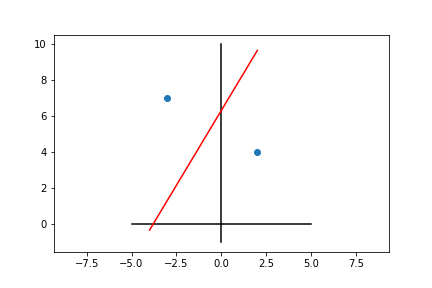
\includegraphics[width = 0.7\linewidth]{fig/pblm2_7}
	\caption{Visualization of the boundary for the halfspace.}
	\label{fig:pblm2_7}
\end{figure}


%\newpage
\subsection{Problem 2.12}
\textbf{Problem:}\\
Which of the following sets are convex?\\

\noindent
\textbf{Solution:}
\subsubsection{(a) - Slab}
A slab defined as $$\{x \in \real^n \ | \ \alpha \leq a^T x \leq \beta\}$$ \textbf{is convex} as it consists of the intersection of two halfspaces which themselves are complex.

\subsubsection{(b) - Rectangle/Hyperrectangle}
A rectangle set defined as $$\{x \in \real^n \ | \ \alpha_i \leq x_i \leq \beta_i, \ i = 1,\dots,n\}$$ \textbf{is convex} as it is composed of the intersections of half spaces which are themselves convex. This is similar to the polyhedrons/polytopes that by definition are also convex.

\subsubsection{(c) - Wedge}
A wedge set given as $$\{x \in \real^n \ | \ a_1^T x \leq b_1, a_2^T x \leq b_2\}$$ \textbf{is convex} as it is just an intersection of two halfspaces (a polyhedron).

\subsubsection{(d) - Closer to a point then a set}
A set of points closer to a given point than a given set is defined as $$\{x \| \norm{x-x_0}_2 \leq \norm{x - y}_2 \ \forall y \in S\}$$ where $S\subset\real^n$ \textbf{is not convex} in general. This is because there is not enough information about $y$ for a conclusion to be made whether it is convex or not. A counter example would be if $y$ is a point in orbit around a convex shape $S$ that would end up generating a concave $x$.

\subsubsection{(e) - Closer to a set then another set}
A set of points closer to a given set than another given set is defined as $$\{x \ | \ \textbf{dist}(x,S) \leq \textbf{dist}(x,T)\}$$ where $S, T \subset\real^n$, and $$\textbf{dist}(x,S) = \inf\{\norm{x-z}_2 \ | \ z \in S\}$$ \textbf{is not convex} in general. This is because there is not enough information about $S$ and $T$ for a conclusion to be made whether it is convex or not. A counter example includes if $S$ or $T$ themselves are a concave shave that causes the set $x$ to also be concave and therefore not convex.


\subsubsection{(f) - Set of the sum being within a convex set}
The set defined as $$\{x \ | \ x + S_2 \subset S_1\}$$ with $S_1$ being convex \textbf{is }\\

??????????????????????????????????????\\

\subsubsection{(g) - Set with weighted distances to two points}
The set of all points that is closer to $a$ then $b$ by at least a factor of $\theta$, defined as $$\{x \in \real^n \ | \ \norm{x-a}_2 \leq \theta \norm{x-b}_2\}$$ with $a \neq b$ and $0 \leq \theta \leq 1$ \textbf{is convex.} This is know because, as proven in a previous problem, a hyperplane is formed for a similarity stated problem which itself is convex. When the distance to $a$ must be less then a portion of the distance to $b$ it will cause the psudo-hyperplane to curve inwards and untimely remain convex.


\newpage
\subsection{Problem 2.28}
\textbf{Problem:}\\
Define the positive semi-definite cone ($S_+^n$) for $n = 1, 2, 3$ in terms of ordinary inequalities with the matrix coefficients themselves.

\noindent
\textbf{Solution:}\\
The positive semi-definite cone is defined for size $n$ as the set of all symmetric matrices that are positive semi-definite:
\begin{equation}
	S_+^n \equiv \{x \in S^n \ | \ x \succeq 0\}
\end{equation}
One method to ensure that a matrix is positive semi-definite is to ensure that its leading principle minors are all non-negative (strictly positive for positive definite).\\

For $n=1$ the required inequalities are simple, 
\begin{equation}
	X = \mqty[x_1] \in S_+^1 \iff x_1 \geq 0
\end{equation}

For $n=2$ the inequalities can be found by ensuring the leading principle minors are all non negative:
\begin{equation}
	\begin{aligned}
		m_1 &= \det[x_1]\\
		&= x_1\\
		m_2 &= \det \mqty[x_1 & x_2 \\ x_2 & x_3] \\
		&= x_1 x_3 - x_2^2
	\end{aligned}
\end{equation}
These definitions of the minors can be then be used to construct inequalities such that all the minors are positive:
\begin{equation}
	X = \mqty[x_1 & x_2 \\ x_2 & x_3] \in S_+^2 \ \iff \ \mqty{x_1 \geq 0\\  x_1 x_3 \geq x_2^2}
\end{equation}

For $n=3$ the inequalities can be found by ensuring the leading principle minors are all non negative:
\begin{equation}
	\begin{aligned}
		m_1 &= \det[x_1]\\
		&= x_1\\
		m_2 &= \det \mqty[x_1 & x_2 \\ x_2 & x_4] \\
		&= x_1 x_4 - x_2^2\\
		m_3 &= \det \mqty[x_1 & x_2 & x_3\\ x_2 & x_4 & x_5\\ x_3 & x_5 & x_6] \\
		&= x_1 (x_1 x_4 - x_2^2) - x_2 (x_2 x_6 - x_3 x_5) + x_3 (x_2 x_5 - x_3 x_4)\\
		&= x_1^2 x_4 - x_1 x_2^2 - x_2^2 x_6 + x_2 x_3 x_5 + x_2 x_3 x_5 - x_3^2 x_4
	\end{aligned}
\end{equation}
These definitions of the minors can be then be used to construct inequalities such that all the minors are positive:
\begin{equation}
	X = \mqty[x_1 & x_2 & x_3\\ x_2 & x_4 & x_5\\ x_3 & x_5 & x_6] \in S_+^2 \ \iff \ 
	\mqty{x_1 \geq 0\\
			x_1 x_4 \geq x_2^2\\
		 x_1 x_2^2 + x_2^2 x_6 + x_3^2 x_4 \geq x_1^2 x_4 + 2 x_2 x_3 x_5}
\end{equation}


%For $n=2$ the inequalities can be found by first calcualting the eigenvalues:
%\begin{align}
%	X &= \mqty[x_1 & x_2\\ x_2 & x_3]\\
%	\intertext{The charectoristic polynomial is then given as:}
%	\det(sI-X) 	&= (s-x_1)(s-x_3) - x_2^2\\
%				&= s^2 - (x_1 + x_3)s + x_1 x_3 - x_2^2\\
%	\intertext{The roors of the charectoristic polynomial represent the eigenvalues:}
%	\lambda_{1,2} 	&= \cfrac{(x_1 + x_3) \pm \sqrt{(x_1 + x_3)^2 - 4 (1)(x_1 x_3 - x_2^2)}}{2}\\
%					&= \cfrac{x_1 + x_3 \pm \sqrt{x_1^2 + x_1 x_3 + x_3^2 - 4 x_1 x_3 + 4 x_2^2}}{2}
%\end{align}


\subsection{Problem 2.33}
\textbf{Problem:}\\



\textbf{Solution:}\\





\section{Problem Set 2: Convex Functions}

\subsection{Problem 3.6}
\textbf{Problem:}\\



\textbf{Solution:}\\


\subsection{Problem 3.16}
\textbf{Problem:}\\



\textbf{Solution:}\\


\subsection{Problem 3.18a}
\textbf{Problem:}\\



\textbf{Solution:}\\


\subsection{Problem 3.22}
\textbf{Problem:}\\



\textbf{Solution:}\\


\end{document}
